
\subsubsection{Reliability Analysis}
\label{subsec:reliability}

We now analyze and place our model in a reliability theory framework. 
%

\noindent \textbf{Expected Lifetime.} Our analytical model helps crystallize the differences in VM preemption dynamics, by allowing us to easily calculate their expected lifetime. 
More formally, we define the expected lifetime of a VM ($\mathscr{L}$) as: 
\begin{equation}
  \label{eq:expected-lifetime}
E[\mathscr{L}] =  \int_{0}^{L} t {f}(t)~dt =  -A(t+\tau_1)e^{-t/\tau_1} + A(t-\tau_2) e^{\frac{t-b}{\tau_2}} \biggr\rvert_{0}^{L}
%E[\mathscr{L}] =  \int_{0}^{L} t {f}(t)~dt 
\end{equation}
where $f(t)$ is the rate of preemptions of the VM (Equation~\ref{eq:failrate}).
%= \dfrac{d \mathscr{F}(t)} {dt} = A \left(\dfrac{1}{\tau_1}e^{-t/\tau_1} + \dfrac{t-b}{\tau_2}e^{\frac{t-b}{\tau_2}}\right) $ 
%
%Since preemptions require restarting a job and increase the job completion time, it may be more prudent to select transient VMs with higher expected lifetimes.
%
This expected lifetime can be used in lieu of MTTF, for policies and applications that require a ``coarse-grained'' comparison of the preemption rates of servers of different types, which has been used for cost-minimizing server selection~\cite{flint}. 

%We use the analytically derived expected lifetimes of VMs of different types in \sysname when selecting the ``best'' VM type for a given bag of jobs. This server selection is a key part of \sysname design. 

\noindent \textbf{Hazard Rate.}
The hazard rate $\lambda(t)$ governs the dynamics of the failure (or survival) processes. It is generally defined as $\lambda(t) = \frac{f(t)}{S(t)}$ and often expressed via the following differential equation (rate law):
\begin{equation}\label{eq:hazard}
\frac{dS(t)}{dt} = -\lambda(t) S(t),
\end{equation}
%$\lambda(t) = \frac{f(t)}{S(t)}$ \vikram{this was inverted, I fixed. double check please}, 
where $S(t) = 1 - F(t)$ is the survival function associated with a CDF $F(t)$, and $f(t)=dF(t)/dt$ is the failure probability function (rate) at time $t$. The survival function indicates the amount of VMs that have survived at time $t$.
The hazard rate can also be directly expressed in terms of the CDF as follows: $1-F(t) = \exp{\int_0^t{-\lambda(x) ~dx}}$. 
The exponential distribution has a constant hazard rate $\lambda$.
The Gompertz-Makeham distribution has an increasing failure rate to account for the increase in mortality, and its hazard rate is accordingly time-dependent and given by $\lambda(t) = \lambda + \alpha e^{\beta t}$.

Since we model multiple failure rates and deadline-induced preemptions, our hazard rate is expected to increase with time. Defining the survival function for our model: $S = 1 - \mathscr{F}$, and using Eq.~\ref{eq:hazard} yields the hazard rate associated with our model: 
%$\lambda(t) = \dfrac{- r_1 e^{- r_1 t} - r_2 e^{r_2 (t - b)}}{e^{- r_1 t} - e^{r_2 (t - b)}}$. 
% missing minus sign in the above equation
\noindent 
\begin{equation}
  \label{eq:hmodel}
  \lambda %= r_2 + \bar{r} \left( \dfrac{1}{1 - e^{- r_2 b} e^{\bar{r} t}}\right)
  %= \dfrac{r_1 + r_2 e^{- r_2 b} e^{\bar{r} t}}{1 - e^{- r_2 b} e^{\bar{r} t}}.  
  = \dfrac{r_1 e^{- r_1 t} + r_2 e^{r_2 (t - b)}}{1/A - 1 + e^{- r_1 t} - e^{r_2 (t - b)}}
\end{equation}
where we have introduced $r_1 = 1/\tau_1$, $r_2 = 1/\tau_2$ to denote the rates of preemptions associated with initial and final phases respectively.

%\vikram{without the A term, hazard rate becomes negative for the older expression you had when $t > b r2 / (r1+r2)$. that is for t roughly greater than b/2, which is for more than 12 hours. hazard rate can never be negative.}
%Here we have introduced the sum of the two failure rate constants, $\bar{r} = r_1 + r_2$, to simplify the expression. \vikram{check}

%Employing the value for $A$ resulting from ensuring (via fit or by force) that our CDF goes to 1 at $t = L$ (where $L$ is 24 hours), we find

% \begin{equation}
%   \label{eq:hmodel2}
%   \lambda %= r_2 + \bar{r} \left( \dfrac{1}{1 - e^{- r_2 b} e^{\bar{r} t}}\right)
%   %= \dfrac{r_1 + r_2 e^{- r_2 b} e^{\bar{r} t}}{1 - e^{- r_2 b} e^{\bar{r} t}}.  
%   = \dfrac{r_1 e^{- r_1 t} + r_2 e^{r_2 (t - b)}}{e^{r_2 (L - b)}  - e^{- r_1 L} + e^{- r_1 t} - e^{r_2 (t - b)} }
% \end{equation}

Recall that the sharp increase in preemption rate only happens close to the deadline, which means that $b \lesssim L$. Thus, when $0 < t \ll b$, we get $\lambda(t) \approx r_1$, mimicking the hazard rate for the classic exponential distribution.
As $t$ approaches and exceeds $b$ (i.e., $b\lesssim t < L$), the increase in the hazard rate due to the second failure process kicks in, accounting for the deadline-induced rise in preemptions. Note that our hazard rate satisfies $\lambda(t) \ge 0$ for $0<t<L$.

% For ease of exposition, we can write this as:

% \begin{equation}
%  \label{eq:hmodelsimple}
% \lambda =  \dfrac{r_1 + \gamma_1 e^{\delta (t-b)}}{1 - \gamma_2 e^{\delta (t-b)}}
% \end{equation}
% 
% We note that the numerator is  similar to the hazard rate associated with Gompertz-Makeham distribution.
% The key difference is the $1-\gamma_2 e^{t-b}$ factor in the denominator. 
% Recall that the sharp increase in preemption rate only happens close to the deadline, which means that $b \leq 24$. Thus, when $t < b$, we get a conventional $\lambda = r_1$, or the classic exponential distribution.
% As $t$ approaches and exceeds $b$, the increase in failure rate kicks in, accounting for the deadline-driven rise in preemptions. 



\subsection{Statistical mechanics of constrained preemptions}
\label{subsec:stat-mech}

For constrained preemptions, one might expect to see uniformly distributed preemptions with a probability $1/L$ over $[0, L]$. 
However, as our empirical analysis shows, the preemption distribution is bathtub-shaped.
Interestingly, we can show using exact analytical arguments that non-uniform, bathtub distributions are in fact an \emph{emergent} characteristic of systems with constrained preemptions, modulo some assumptions. 

\begin{lemma}\label{lemma:1}
  Consider $N$ randomly distributed preemptions over an interval $[0, L]$.
  Assume that each preemption takes $w > 0$ time-units to perform, and preemptions cannot overlap, i.e, they occur in a mutually exclusive manner.
  Then, there exists $\epsilon > 0$ such that  $P(L-\epsilon) > \frac{1}{L}$, where 
 $P(t)$ is the probability of finding a preemption at time $t$. 
\end{lemma}


\begin{proof} 
We first make some preliminary remarks and introduce concepts necessary to complete the proof. 

Firstly, mutual exclusion of preemptions implies that there is a finite non-zero waiting time $w>0$ between preemptions. 
For $N$ preemptions to occur within $L$ interval, evidently, we must have $N w < L$. Also, while $w >0$, the time to perform the preemption is generally expected to be much smaller than the total time interval $L$ (i.e., $w \ll L$).
$N$ preemptions occupy a ``temporal volume'' of $Nw$ (volume here represents the one-dimensional volume). We assume that while a preemption may start at $t=0$, the last preemption must finish by $t = L$. Thus, the amount of free or excluded ``temporal volume'' available within the constrained system is $L_e = L - w - (N-1)w = L - Nw$.
%The concept of excluded volume arising due to the finite-size of the particles is central to understand the physics of material systems in confined environments and is explain the origin of steric forces and correlations \cite{krauth2006statistical,jing2015ionic,solis2013generating}. 
We note that the concept of excluded volume is routinely employed in the analysis of physical systems such as liquids and polymers, where the excluded volume of particles acts as a constraint that gives rise to steric forces and structural changes in material behavior \cite{krauth2006statistical,jing2015ionic,solis2013generating}. 

Secondly, we observe that the system of $N$ preemptions within a constrained deadline of interval $L$ maps \emph{exactly} to a well known and analytically solvable system in classical statistical mechanics, the one-dimensional Tonks gas model \cite{tonks}. The Tonks gas model describes a system of $N$ non-overlapping particles of finite size $w$ that are constrained to move within a line segment of length $L$. The structural quantities associated with this system, including the probability of finding a particle at position $x$ within the spatial confinement of length $L$, are computed by evaluating the partition function of the system, which essentially measures the number of valid system configurations \cite{krauth2006statistical}. 
%below para is not clear to me; i add my suggestion below it
%Employing this mapping and the associated statistical mechanics tools, the original model of non-overlapping (interacting) preemptions can be mapped to a system of $N$ overlapping (non-interacting) preemptions, each allowed to access an excluded volume of $L_e$, and the number of valid configurations is given by the partition function $Z_N = L_e^N$. For the case of $N$ preemptions, we have $Z_N = (L- Nw)^N$.
Employing this mapping, we consider a system of $N$ non-overlapping preemptions constrained within a ``time confinement'' of size $L$. Each preemption has access to an excluded volume of $L_e$ within this constrained system. 
The number of ways $N$ preemptions can occur within the interval $L$ is equivalent to the number of valid configurations for this system, which is given by its partition function: $Z_N = L_e^N = (L- Nw)^N$.

We are interested in calculating the probability that a preemption starts at time $t=L-w$, i.e., $P(L-w)$. Given $w \ll L$, $P(L-w)$ is the probability of finding a preemption near the deadline. The assumption of mutually exclusive preemptions implies that no other preemption can be found for $t > L - w$, that is, $P(t> L-w) = 0$. Hence, the remaining $N-1$ preemptions must occur such that the last of those finish by $t=L-w$. In other words, the preemption at time $L-w$ essentially sets an effective deadline for the other $N-1$ preemptions. The number of ways those $N-1$ preemptions can happen within the time interval of $L-w$ is given by the partition function $Z_{N-1} = L_e^{N-1}= (L-2w - (N-2)w)^{N-1} = (L - Nw)^{N-1}$, where $L_e = L - Nw$ is the corresponding excluded temporal volume available to each of the $N-1$ preemptions.
It is interesting to note that this excluded volume
%in this case
is the same as that of the original $N$ preemption system: this fortuitous result arises because the decrease in the available volume (``time confinement'') to place the preemptions is commensurate with the need to place fewer ($N-1$) preemptions.

The probability $P(L-w)$ is obtained as the ratio of the valid configurations given by the two partition functions computed above.
%That is, $P(L-w) = Z_{N-1}/ {Z_N} = \frac{1}{L - Nw} > \frac{1}{L}$ , since $N \geq 1$ and $w>0$. Choosing $\epsilon = w > 0$ completes the proof.
That is, $P(L-w) = Z_{N-1}/ {Z_N} = \frac{1}{L - Nw}$. Because $N \geq 1$ and $w>0$, we find $P(L-w) > \frac{1}{L}$. Choosing $\epsilon = w$ completes the proof.
\end{proof}

By symmetry arguments, the above lemma is in fact valid for both the end points of the interval, i.e., $P(\epsilon) > \frac{1}{L}$.
In other words, the probability of preemption is higher near the end points (deadline) than the average preemption probability of $1/L$, and we get a bathtub shaped distribution.
For the above proof, we assumed that each preemption event occurs over a timespan of $w$, which is determined by the preemption warning that the cloud platform provides (which is 30 seconds for Google Preemptible VMs and 120 seconds for Amazon EC2 spot instances). 
Preempting a VM and reclaiming its resources involves manipulating the cluster-management state, and mutually exclusive preemptions may be convenient for cluster management, since serializing VM preemptions makes accounting and other cluster operations easier.
From an application standpoint, non-overlapping preemptions are also beneficial, since handling multiple concurrent preemptions is significantly more challenging~\cite{exosphere}. 



Thus, statistical mechanics indicates that the bathtub distribution follows from the constrained and non-overlapping nature of preemptions, if we assume no other external factors or cloud policies influencing the preemptions. 
%To validate this, we conduct a monte carlo simulation of temporally constrained and non-overlapping preemptions. 
Figure~\ref{fig:partfun} shows the preemption probability computed using the partition function.
We find that this probability \emph{also} follows the bathtub shape that is found in the empirical data. 


%Of course, the empirical preemption distribution is determined by the cloud platform's policies and supply and demand.
%, and we elaborate more about the generality of our model and observation in Section~\ref{sec:discussion}. \vikram{will we add discussion at the end?}

% How ?
%Crucial to our The assumption of preemption events

\begin{figure}[t]
  \centering
  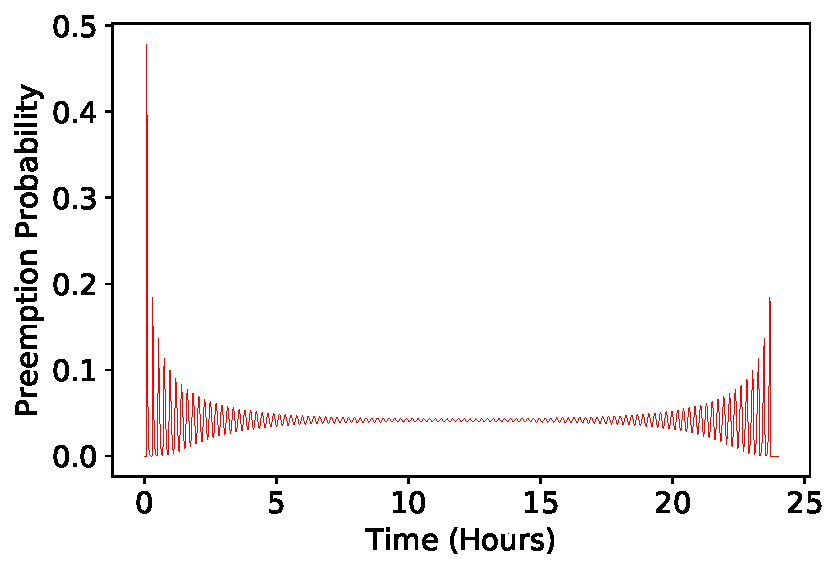
\includegraphics[width=0.3\textwidth]{../graphs/analytical_prob.pdf}
  \caption{Preemption probability computed using the partition function defined for a simple constrained system is also bathtub shaped.}
  \label{fig:partfun}
\end{figure}

 


%%% Local Variables:
%%% mode: latex
%%% TeX-master: "paper"
%%% End:
